\section{Comparative analyses of simulation results}

At the start of our different comparative analyses, we will first make some general rough analysis, thereby creating a more simplified and easy-to-understand version of our results. As an example, in figure \ref{fig:peak_infected}, two histograms are visible, showcasing the only difference in the underlying simulation, which is the switching of contact tracing (CT). 

In the first histogram, the columns clearly shows the effect of contact tracing. The maximum number of total infected within thousand drops of our simulation shows no higher than 210 infected of a total 12,500 population size, which equals to 1.68\% being infected of a total population. In other words, this is a very low total infection. 
-
\begin{figure}[H]
  \centering
  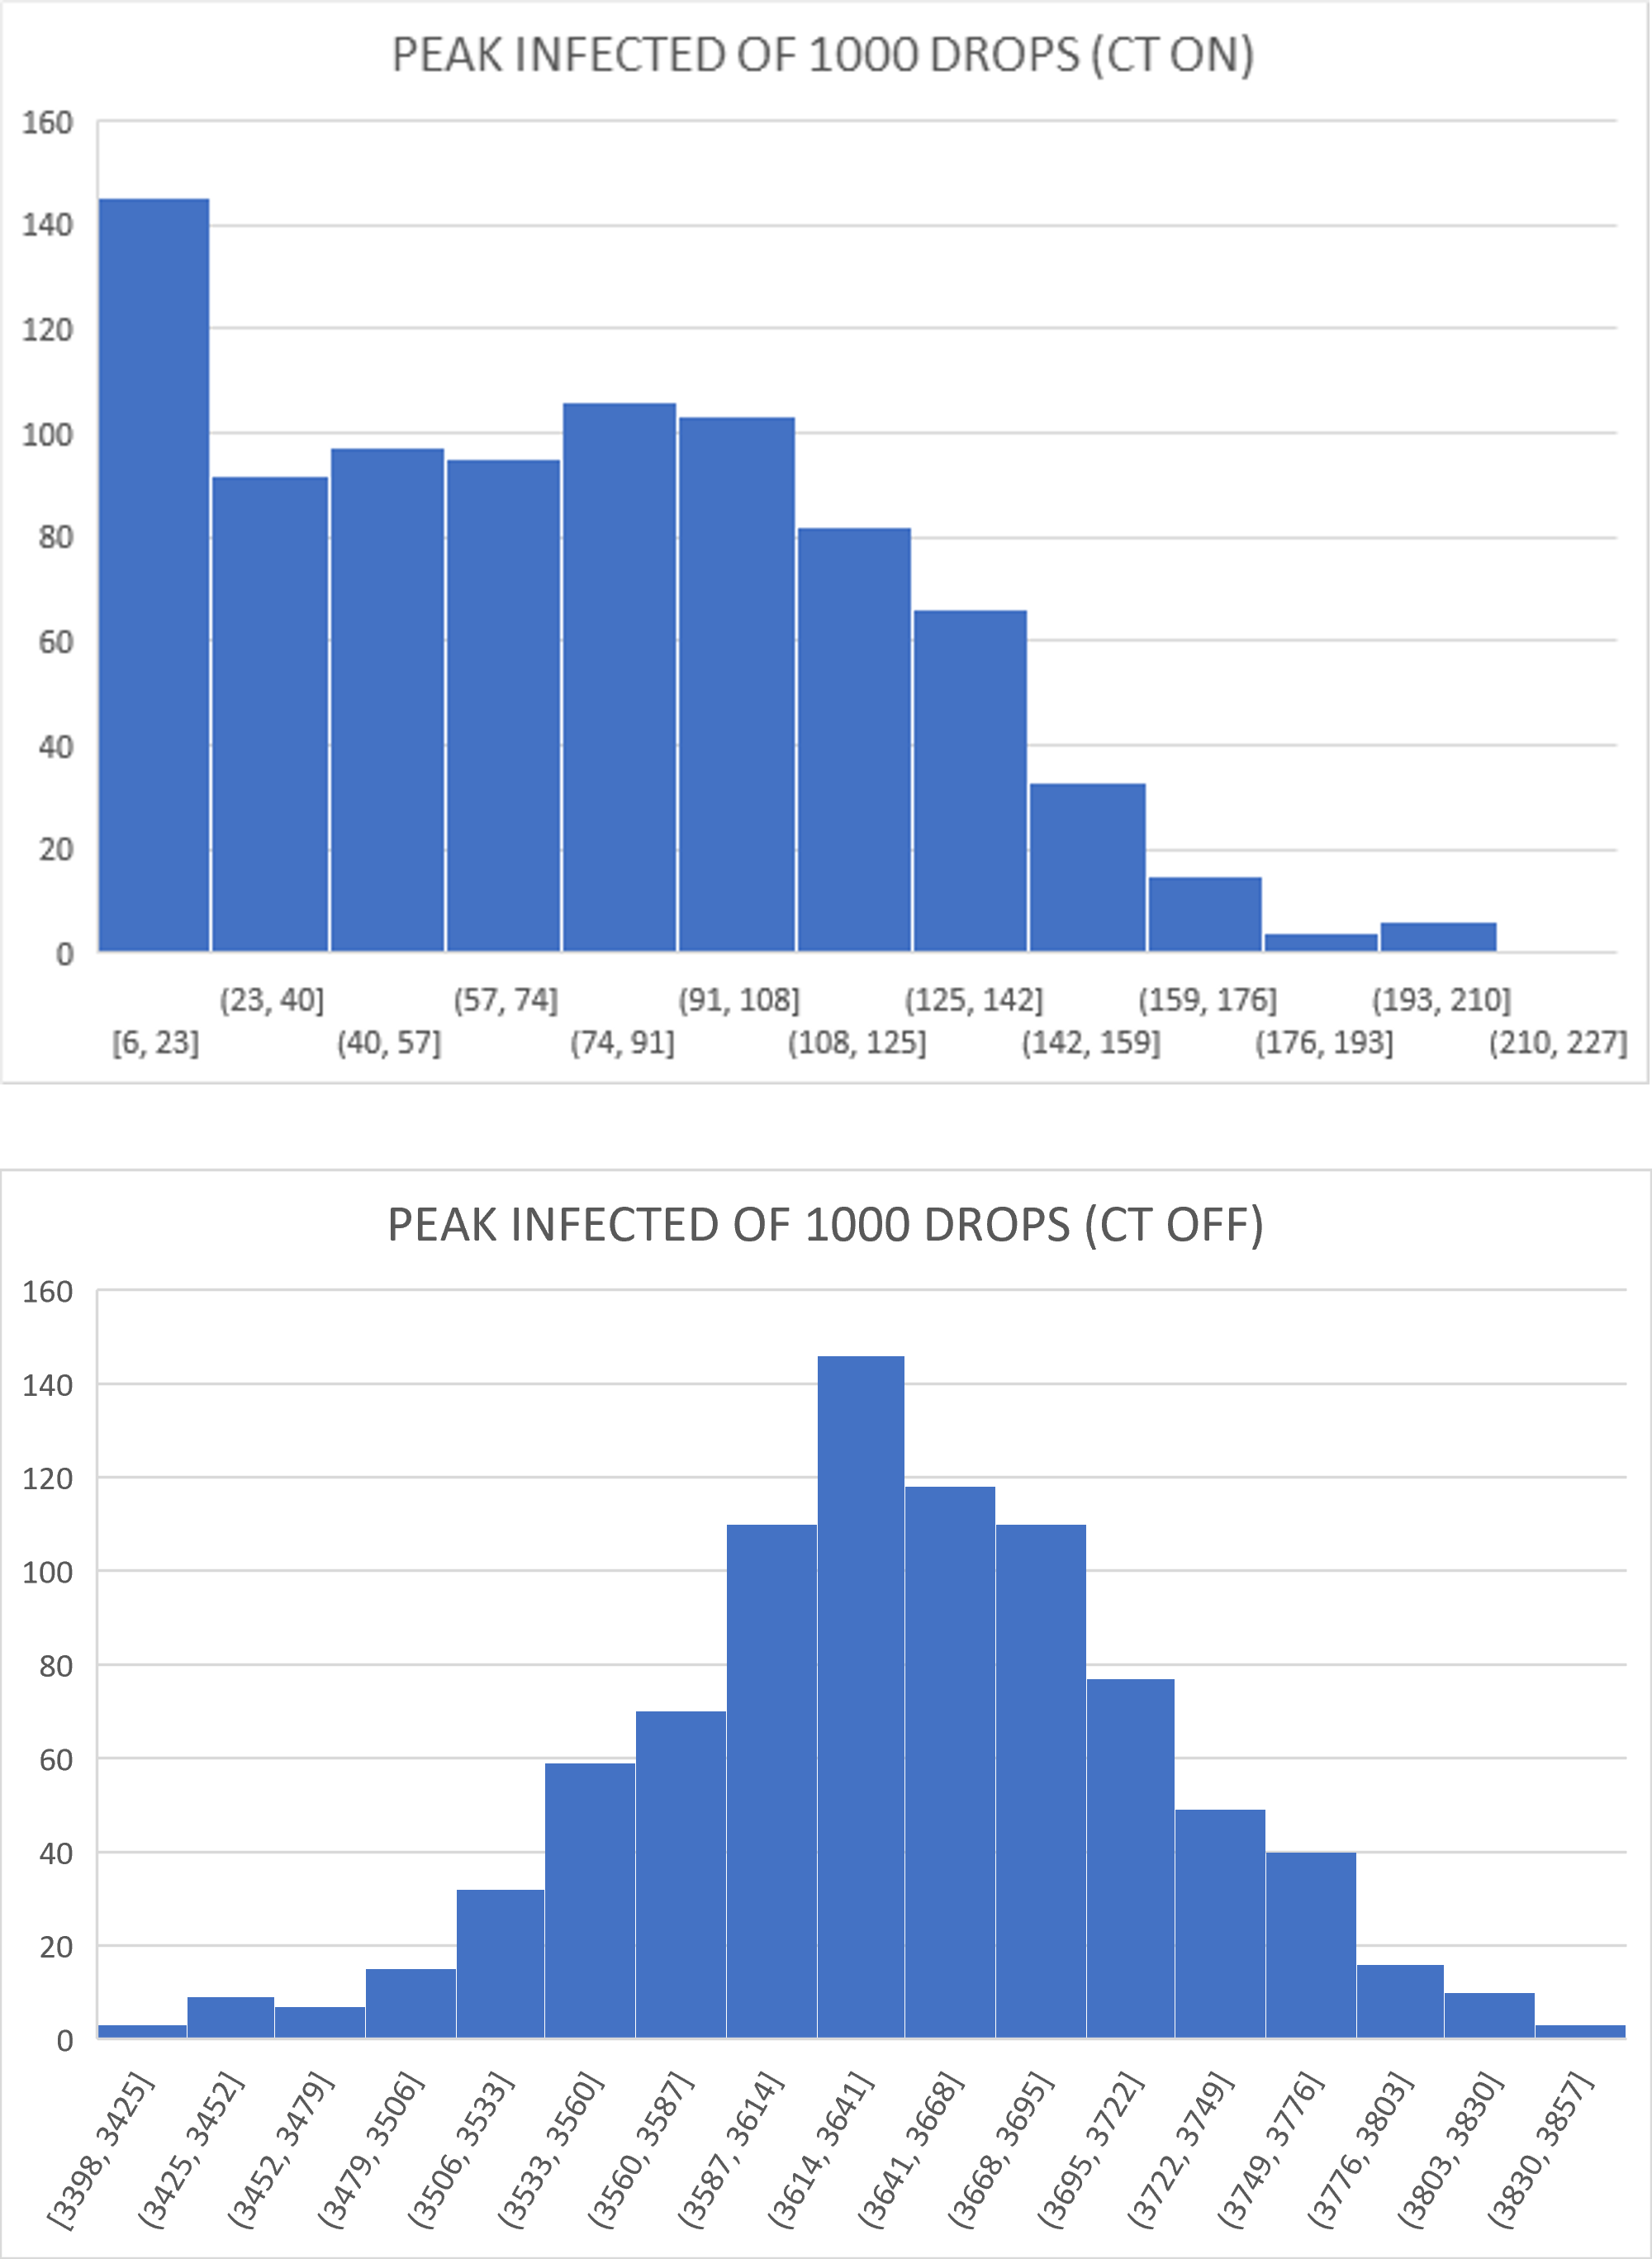
\includegraphics[width=\textwidth]{0_billeder/Peak_infected_graph.png}
  \caption{Histogram of peak infected, with (upper) and without contact tracing (lower) graph.}
  \label{fig:peak_infected}
\end{figure}


Figure \ref{Fig:covidInfGraphs} is a graph of infection, as a function of days, both with- and without contact tracing enabled. Before going into explaining the graphs, it is important to note, that the data used is an average of a thousand drops.

In the first graph with contact tracing disabled, we see that the number of infected people is raising rapidly to its peak which is around 2750 people infected - at day 112. Then the number of infected people quickly drops to 0 again around day 190 and do not change further.

In the second graph, which is with contact tracing enabled, the number of infected also raises rapidly, but it does not reach the same levels as in the first graph. The maximum number of infected in the second graph is around 33 at day 140. After it has peaked, it slowly decrease towards 0, which is reached around day 720.

Comparing the two, it is clearly that contact tracing and quarantine is a very effective tool in fighting COVID-19. With contact tracing disabled, the number of infected people peak at 2750 people, whereas with contact tracing enabled, it peaks at only 33 infected people. That corresponds to only 1.2\% of the first graph's peak.

\begin{figure}[H]
  \centering
  
  \begin{subfigure}{.45\textwidth}
    \centering
    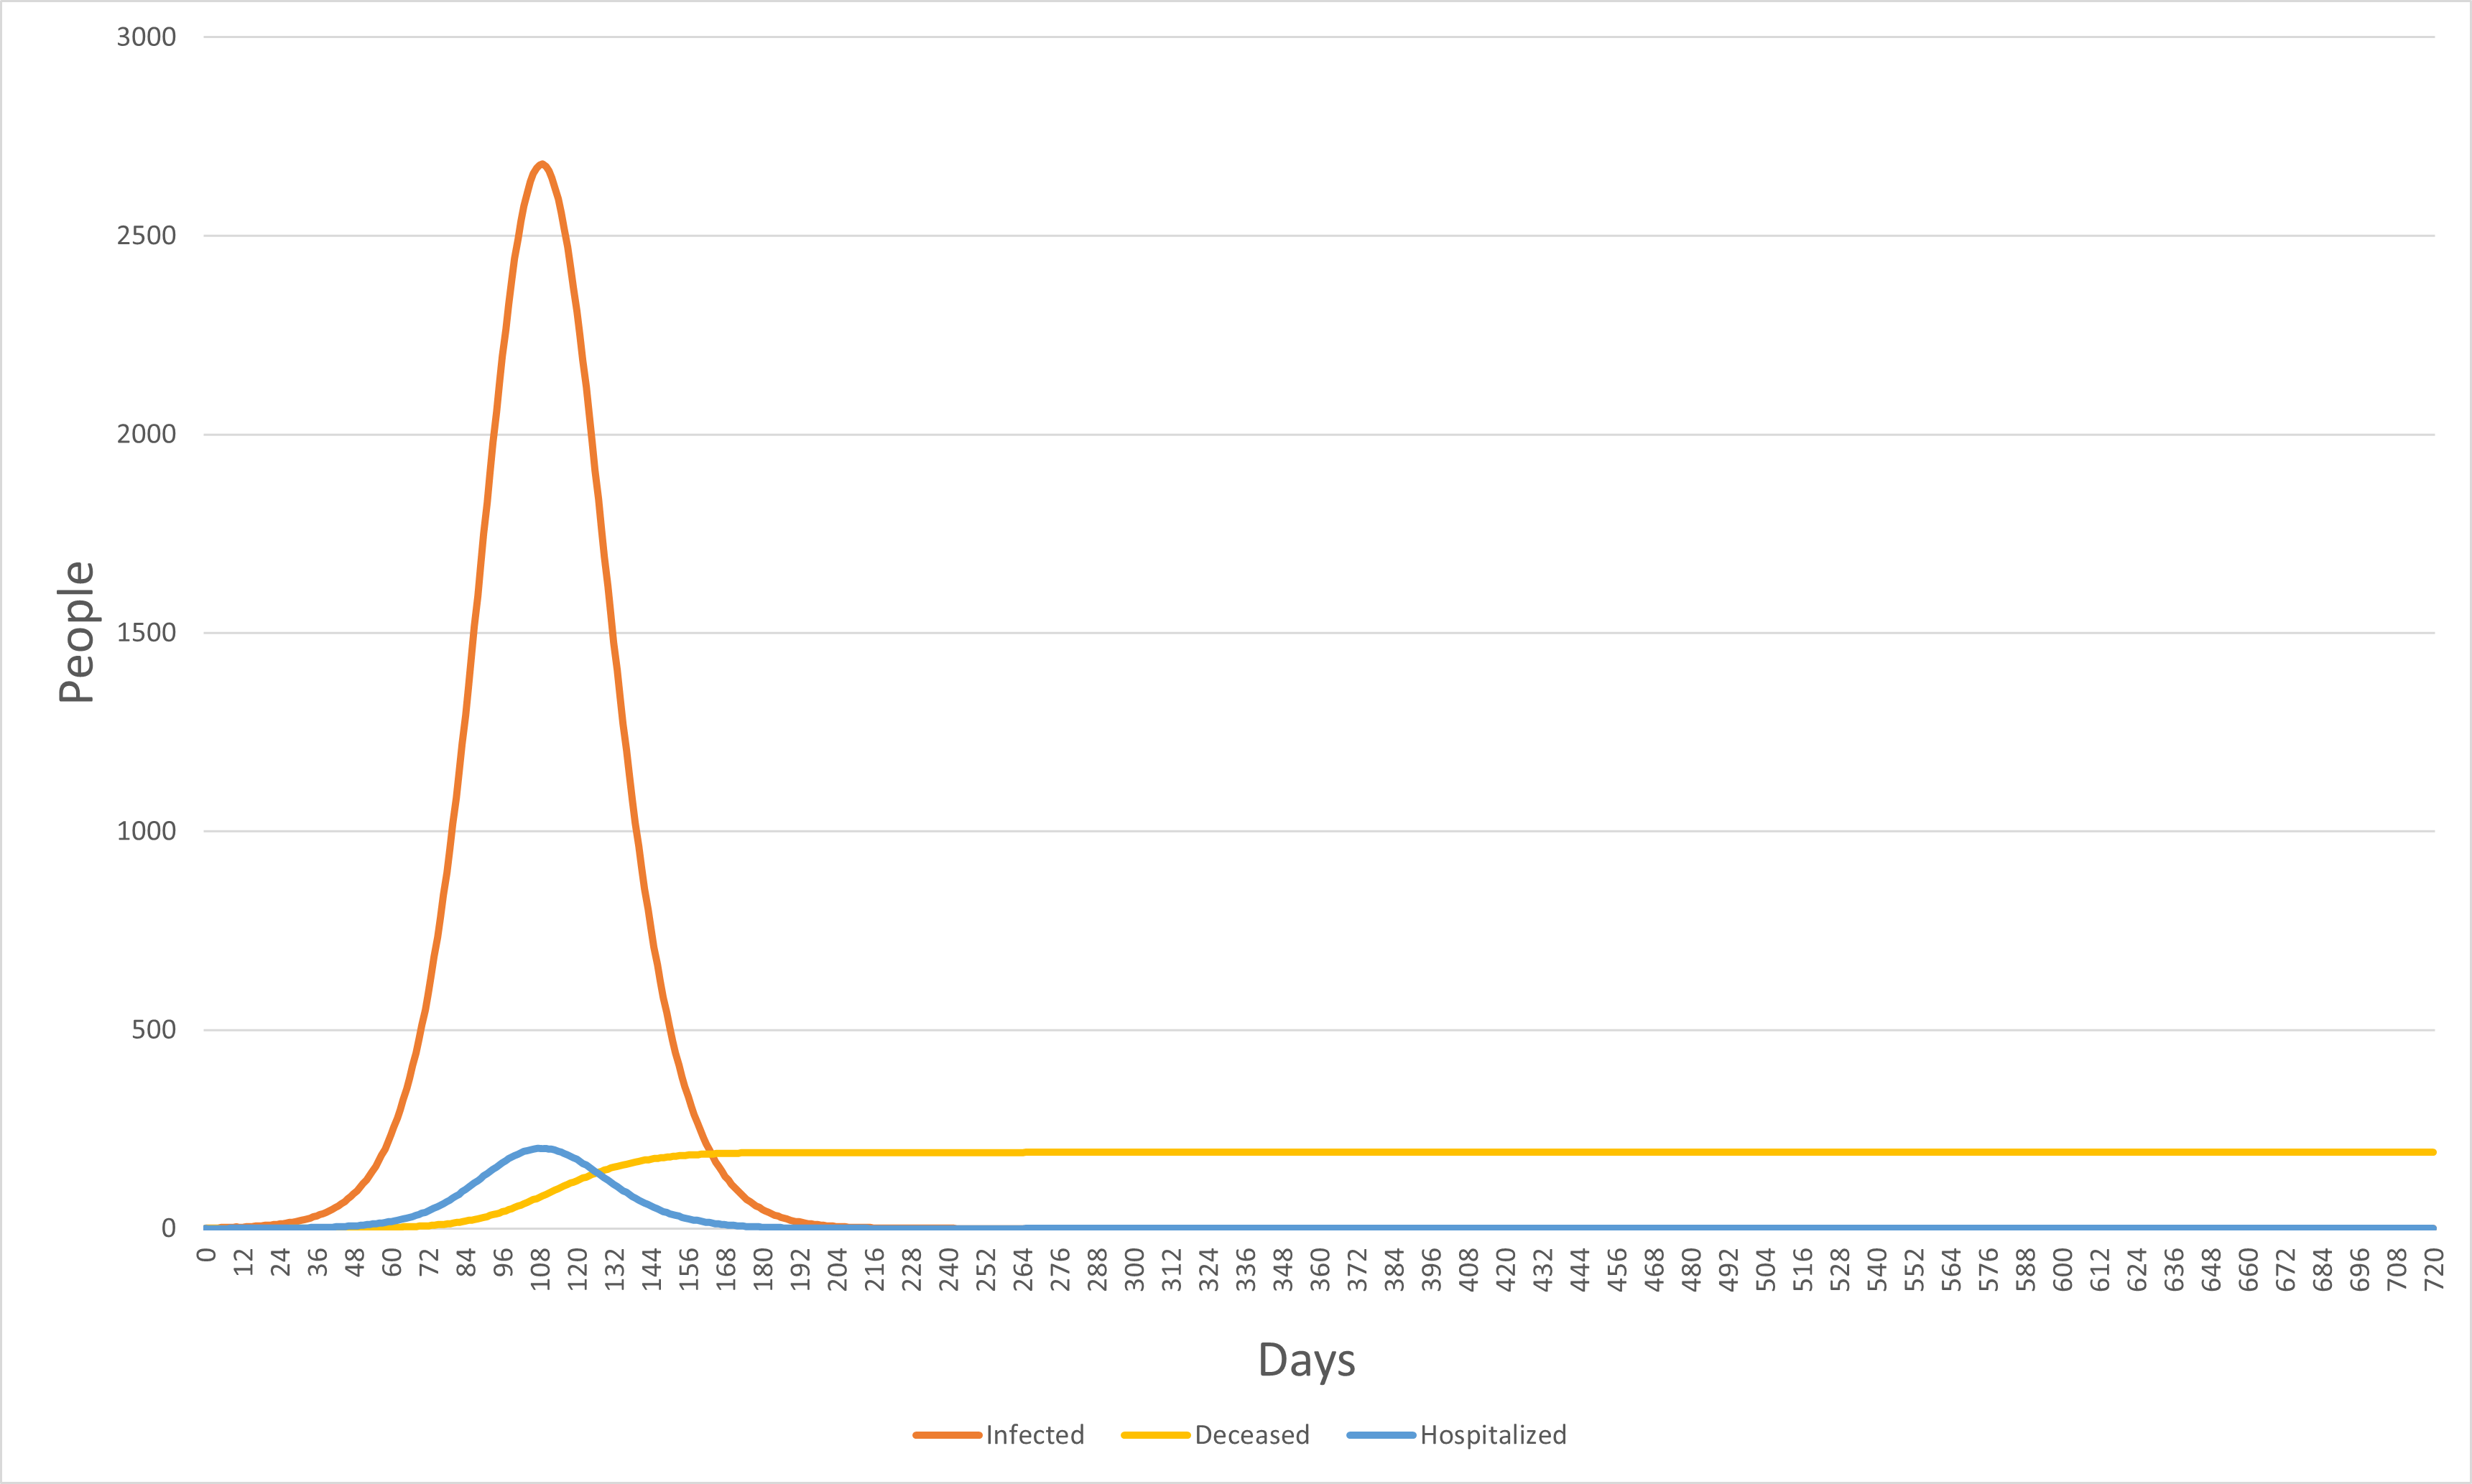
\includegraphics[width=.95\linewidth]{0_billeder/covidInfectionGraphA.png}
    \caption{Graph of infection, with contact tracing enabled}
    \label{Subfig:covidInfGraphA}
  \end{subfigure}
  
  \begin{subfigure}{.45\textwidth}
    \centering
    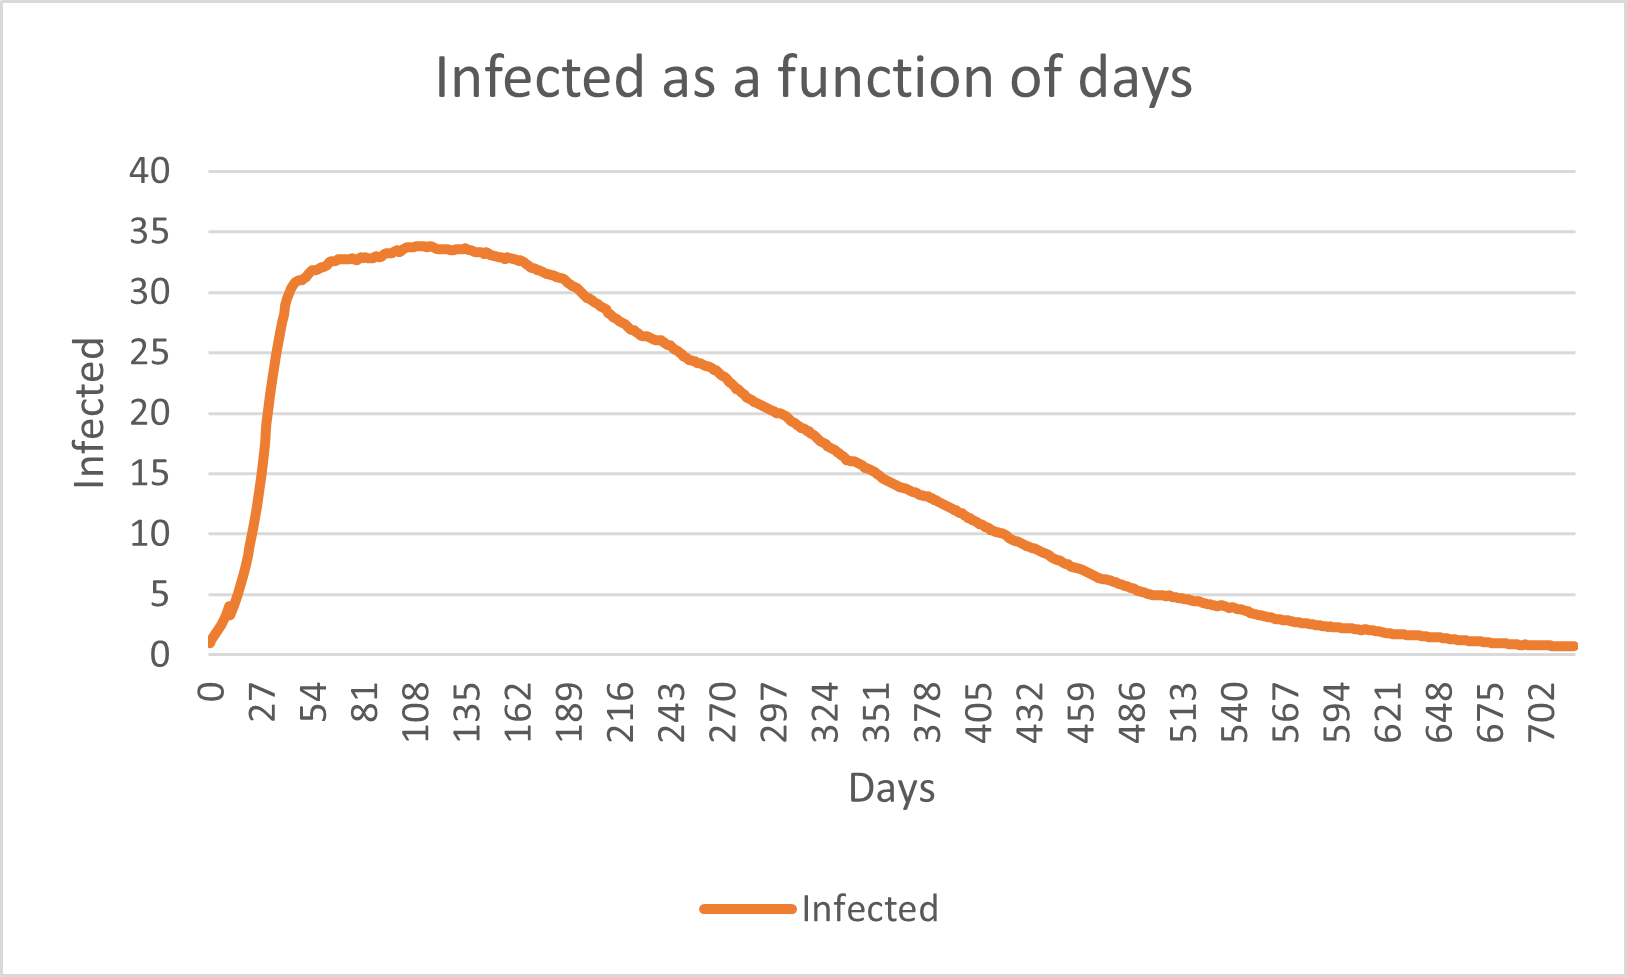
\includegraphics[width=.95\linewidth]{0_billeder/covidInfectionGraphB.png.png}
    \caption{Graph of infection, with contact tracing disabled}
    \label{Subfig:covidInfGraphB}
  \end{subfigure}
  \label{Fig:covidInfGraphs}
  
\end{figure}



%\subsection{Results Expressed in Histogram}

%Maybe maybe not

%\subsection{Detailed Analysis}

%Mere dybdegående analyse af forskelle + ligheder her

%\subsection{Real Life Data Comparison}

%


